\documentclass[aspectratio=43,9pt]{beamer}
%
\usepackage{tikz}
\usepackage{enumerate}
\usepackage{setspace}
%
\usetheme{Boadilla}
%
\graphicspath{{./figures/nt3/}}
%
\let\Tiny=\tiny%			% to avoid warnings about font size
%\usepackage{lmodern}%		% alternative method to avoid these warnings
%
\catcode`~=11 % make LaTeX treat tilde (~) like a normal character
\newcommand{\urltilde}{\hbox{~}}
\catcode`~=13 % revert back to treating tilde (~) as an active character
%
% misc commands
\newcommand{\bm}[1]{\mathbf{#1}}
\newcommand{\bs}[1]{\boldsymbol{#1}}
\newenvironment{myitemize}[1]{\vspace{#1}\begin{itemize}\setlength\itemsep{#1}}{\end{itemize}}
%
% pgf markers
\usepgflibrary{plotmarks}
%
\setbeamertemplate{footline}
{
  \leavevmode%
  \hbox{%
  \begin{beamercolorbox}[wd=.8\paperwidth,ht=2.25ex,dp=1ex,left]{author in head/foot}%
    \usebeamerfont{author in head/foot}\hspace*{4em}\inserttitle
  \end{beamercolorbox}%
  \begin{beamercolorbox}[wd=.2\paperwidth,ht=2.25ex,dp=1ex,right]{author in head/foot}%
    \usebeamerfont{author in head/foot}\insertframenumber{} / \inserttotalframenumber\hspace*{1ex}
  \end{beamercolorbox}}%
  \vskip0pt%
}
%
\setbeamertemplate{navigation symbols}{}
%
\setbeamertemplate{frametitle}
{%
	\begin{minipage}{.9\paperwidth}
		\vspace*{1ex}%
		\flushright%
		%\bfseries
		\LARGE%
		\insertframetitle%
	\end{minipage}%
}
%
\setbeamertemplate{title page}{
	\begin{center}
		\vspace*{2ex}
		\usebeamercolor[fg]{frametitle}{%
			\Large%
			Numerical Techniques 2025--2026\\[2ex]
			%
			\LARGE%
			\inserttitle
		}\\[6ex]
		\usebeamercolor[fg]{normal text}{%
			Daan Degrauwe\\[1ex]
			\texttt{daan.degrauwe@meteo.be}\\[4ex]
			Postgraduate Studies in Weather and Climate Modeling\\[1ex]
			Ghent University
		}
	\end{center}
}
%
\newcommand{\ft}[2]{{\textstyle\frac{#1}{#2}}}
%
% increase space around equations
\makeatletter
\g@addto@macro\normalsize{%
	\setlength{\abovedisplayskip}{3ex}%
	\setlength{\belowdisplayskip}{3ex}%
	\setlength{\abovedisplayshortskip}{3ex}%
	\setlength{\belowdisplayshortskip}{3ex}%
}%
\makeatother
%

%
\title{3. Space differencing}%
%
%%%%%%%%%%%%%%%%%%%%%%%%%%%%%%%%%%%%%%%%%%%%%%%%%%%%%%%%%%%%%%%%%%%%%%
%
\begin{document}
%
%%%%%%%%%%%%%%%%%%%%%%%%%%%%%%%%%%%%%%%%%%%%%%%%%%%%%%%%%%%%%%%%%%%%%%%%%%%%%%%%%%%%%%%%%%%%%%%%%%%%
%
\begin{frame}[plain]
	\titlepage
\end{frame}
%
%%%%%%%%%%%%%%%%%%%%%%%%%%%%%%%%%%%%%%%%%%%%%%%%%%%%%%%%%%%%%%%%%%%%%%%%%%%%%%%%%%%%%%%%%%%%%%%%%%%%
%
\begin{frame}
	%
	\frametitle{Previously on Numerical Techniques \ldots}
	%
	\vfill\begin{itemize}
		\item Discretization and finite differences\vfill
		\item Consistency, convergence and stability\vfill
		\item Effects of time discretization on oscillation equation:
			\begin{itemize}
				\item Damping or amplification
				\item Acceleration or deceleration
				\item Implicitness of 2TL schemes
				\item Computational mode of 3TL schemes and filtering
			\end{itemize}
	\end{itemize}\vfill
	%
\end{frame}
%
%
%%%%%%%%%%%%%%%%%%%%%%%%%%%%%%%%%%%%%%%%%%%%%%%%%%%%%%%%%%%%%%%%%%%%%%
%
\begin{frame}
	%
	\frametitle{Waves in space and time}
	%
	\setstretch{1.2}
	%
	The following function is oscillating in space and time:
	%
	\begin{equation*}
		\psi(x,t)=e^{i(kx-\omega t)}
	\end{equation*}
	%
	where
	%
	\begin{itemize}
		\item $\omega$ is the \emph{frequency}: $\omega=\frac{2\pi}{T}$ with $T$ the period;
		\item $k$ is the \emph{wavenumber}: $k=\frac{2\pi}{L}$ with $L$ the wavelength.
	\end{itemize}
	%
	\vspace*{3ex}
	%
	\begin{minipage}{.5\textwidth}
		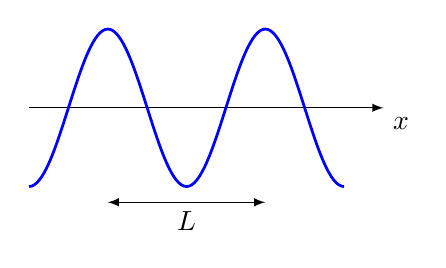
\begin{tikzpicture}[>=latex,x=5mm,y=10mm]
			\draw[->] (-1,0) -- (8,0) node[below right] {$x$};
			\draw[blue,line width=1pt] (-1,-1) cos +(1,1) sin +(1,1) cos +(1,-1) sin +(1,-1) cos +(1,1) sin +(1,1) cos +(1,-1) sin +(1,-1);
			\draw[<->] (1,-1.2) -- (5,-1.2) node[pos=.5,below] {$L$};
		\end{tikzpicture}
	\end{minipage}%
	\begin{minipage}{.5\textwidth}
		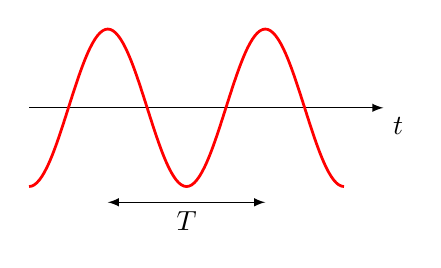
\begin{tikzpicture}[>=latex,x=5mm,y=10mm]
			\draw[->] (-1,0) -- (8,0) node[below right] {$t$};
			\draw[red,line width=1pt] (-1,-1) cos +(1,1) sin +(1,1) cos +(1,-1) sin +(1,-1) cos +(1,1) sin +(1,1) cos +(1,-1) sin +(1,-1);
			\draw[<->] (1,-1.2) -- (5,-1.2) node[pos=.5,below] {$T$};
		\end{tikzpicture}
	\end{minipage}
\end{frame}
%
%%%%%%%%%%%%%%%%%%%%%%%%%%%%%%%%%%%%%%%%%%%%%%%%%%%%%%%%%%%%%%%%%%%%%%
%
\begin{frame}
	%
	\frametitle{The dispersion relation}
	%
	\vfill\begin{itemize}
		\item If $\omega=c\,k$,	then $\psi(x,t)$ is a solution to the advection equation
			%
			\begin{equation*}
				\frac{\partial \psi}{\partial t}+c\frac{\partial \psi}{\partial x}=0
			\end{equation*}\vfill
			%
		\item So there is a relation between the frequency $\omega$ (or period $T$), the wavenumber $k$ (or wavelength $L$) and the propagation speed $c$.\vfill
			%
		\item We call this relation between $\omega$ and $k$ the \emph{dispersion relation}.\vfill
			%
		\item For the advection equation it is simply
			%
			\begin{equation*}
				\omega = c k
			\end{equation*}
			%
			expressing that all waves propagate at the same speed.
			%
	\end{itemize}\vfill
\end{frame}
%
%%%%%%%%%%%%%%%%%%%%%%%%%%%%%%%%%%%%%%%%%%%%%%%%%%%%%%%%%%%%%%%%%%%%%%
%
\begin{frame}
	%
	\frametitle{Group speed and phase speed}
	%
	\vfill\begin{itemize}
		\item We define:\\[2ex]
			\qquad the phase speed $\displaystyle\frac{\omega}k$
			\qquad the group speed $\displaystyle\frac{\partial \omega}{\partial k}$\vfill
			%
		\item For the particular case of the 1D advection equation,\\[2ex]
			group speed $=$ phase speed $=c$.\vfill
			%
		\item Fortran program and Jupyter notebook to illustrate the on HPC:\texttt{/user/gent/407 /vsc40744 /ugent/numtech/lessons/nt3/}
    			%
	\end{itemize}\vfill
\end{frame}
%
%%%%%%%%%%%%%%%%%%%%%%%%%%%%%%%%%%%%%%%%%%%%%%%%%%%%%%%%%%%%%%%%%%%%%%
%
\begin{frame}
	%
	\frametitle{The discrete dispersion relation}
	%
	\vfill\begin{itemize}
		\item we will now determine the dispersion relation when discretizing $x$ (not $t$!): $\omega_d=f(k)$.\vfill
		\item this allows to focus on effect of spatial discretization (cfr. Fourier decomposition to focus on temporal discretization)\vfill
		\item the comparison of the discrete dispersion relation with the exact dispersion relation will tell us\vfill
			\begin{itemize}
				\item amplification: determined by imaginary part of $\omega_d$\vfill
				\item acceleration: determined by real part of $\omega_d$\vfill
			\end{itemize}
			since
			\begin{equation*}
				e^{i\left(k j \Delta x-\omega_d t\right)}=e^{\omega_i t}\,e^{i\left(kj\Delta x-\omega_r t\right)}
			\end{equation*}
	\end{itemize}\vfill
\end{frame}
%
%%%%%%%%%%%%%%%%%%%%%%%%%%%%%%%%%%%%%%%%%%%%%%%%%%%%%%%%%%%%%%%%%%%%%%
%
\begin{frame}
	%
	\frametitle{Dispersion relation with the centered scheme}
	%
	\vfill\begin{itemize}
		\item Let's consider the centered finite difference scheme,
			%
			\begin{equation*}
				\frac{ d \phi_j}{dt} + c 
				\left(
					\frac{\phi_{j+1} - \phi_{j-1}}{2 \Delta x}
				\right)
				= 0
			\end{equation*}\vfill
			%
		\item Suppose the solution is of the form,
			%
			\begin{equation*}
				\phi_j (t) = e^{i \left( k j \Delta x - \omega_{2c} t \right)}
			\end{equation*}\vfill
			%
		\item This will be the case if
			%
			\begin{equation*}
				- i \omega_{2c} \phi_j = - c
				\frac{e^{ik \Delta x} - e^{- i k \Delta x}}{2 \Delta x} \phi_j
			\end{equation*}
			%
			or ($e^{i\theta}=\cos\theta+i\sin\theta$),
			%
			\begin{equation*}
				\omega_{2c} = c \frac{\sin k \Delta x}{\Delta x}
			\end{equation*}
			%
	\end{itemize}\vfill
\end{frame}
%
%%%%%%%%%%%%%%%%%%%%%%%%%%%%%%%%%%%%%%%%%%%%%%%%%%%%%%%%%%%%%%%%%%%%%%
%
\begin{frame}
	%
	\frametitle{Dispersion relation with the centered scheme}
	%
	\vfill\begin{itemize}
		\item $\omega_{2c}$ is real so there is no amplitude error.\vfill
		\item The phase speed is
			\begin{equation*}
				\frac{\omega_{2c}}{k} = c \frac{\sin k \Delta x}{k \Delta x}\approx c \left[1 - \frac16 (k \Delta x)^2\right]
			\end{equation*}
			%
			This is a function of $k$, so the waves are \emph{dispersive}.
			%
			\begin{itemize}
				\item This scheme is second-order in $k \Delta x$.
				\item The phase speed is zero for $k\Delta x = \pi$, i.e. for the ``$2 \Delta x$''-wave.
			\end{itemize}\vfill
			%
		\item The group speed is
			\begin{equation*}
				\frac{\partial \omega_{2c}}{\partial k} = c \cos k \Delta x
			\end{equation*}
			The group velocity of the $2 \Delta x$ waves is $-c$!
	\end{itemize}\vfill
\end{frame}
%
%%%%%%%%%%%%%%%%%%%%%%%%%%%%%%%%%%%%%%%%%%%%%%%%%%%%%%%%%%%%%%%%%%%%%%
%
\begin{frame}
	%
	\frametitle{Higher order scheme}
	%
	\vfill\begin{itemize}
		\item What about a higher-order discretization of $\partial\psi/\partial x$:
			%
			\begin{equation*}
				\frac{d \phi_j}{dt} + c \left[ \frac43 \frac{\phi_{j+1} - \phi_{j-1}}{2 \Delta x} 
					- \frac13 \frac{\phi_{j+2} - \phi_{j-2}}{4 \Delta x} \right] = 0
			\end{equation*}\vfill
			%
		\item Similar calculations give the following discrete dispersion relation:
			%
			\begin{equation*}
				\omega_{4c} = \frac{c}{\Delta x} \left( \frac43 \sin k \Delta x -    \frac16 \sin 2 k \Delta x \right)
			\end{equation*}
			%
			which is fourth-order accurate since the phase speed is
			%
			\begin{equation*}
				c = \frac{\omega_{4c}}{k} \approx c \left[ 1 - \frac{( k \Delta x)^4}{30} \right]
			\end{equation*}
			%
	\end{itemize}\vfill
\end{frame}
%
%%%%%%%%%%%%%%%%%%%%%%%%%%%%%%%%%%%%%%%%%%%%%%%%%%%%%%%%%%%%%%%%%%%%%%
%
\begin{frame}
	%
	\frametitle{Higher order scheme}
	%
	\vfill\begin{itemize}
		\item The group velocity is given by
		%
		\begin{equation*}
			\frac{\partial \omega_{4 c}}{\partial k} =c \left[ \frac43 \cos k \Delta x - \frac13 \cos 2 k \Delta x \right]
		\end{equation*}
		%
		Remark: the $2 \Delta x$ wave has a group velocity of $-\frac53 c$, which is even worse than for the second-order scheme !
	\end{itemize}\vfill
	%
\end{frame}
%
%%%%%%%%%%%%%%%%%%%%%%%%%%%%%%%%%%%%%%%%%%%%%%%%%%%%%%%%%%%%%%%%%%%%%%
%
\begin{frame}
	%
	\frametitle{Scaled frequency}
	%
	\begin{center}
		\scalebox{.8}{% GNUPLOT: LaTeX picture with Postscript
\begingroup
  \makeatletter
  \providecommand\color[2][]{%
    \GenericError{(gnuplot) \space\space\space\@spaces}{%
      Package color not loaded in conjunction with
      terminal option `colourtext'%
    }{See the gnuplot documentation for explanation.%
    }{Either use 'blacktext' in gnuplot or load the package
      color.sty in LaTeX.}%
    \renewcommand\color[2][]{}%
  }%
  \providecommand\includegraphics[2][]{%
    \GenericError{(gnuplot) \space\space\space\@spaces}{%
      Package graphicx or graphics not loaded%
    }{See the gnuplot documentation for explanation.%
    }{The gnuplot epslatex terminal needs graphicx.sty or graphics.sty.}%
    \renewcommand\includegraphics[2][]{}%
  }%
  \providecommand\rotatebox[2]{#2}%
  \@ifundefined{ifGPcolor}{%
    \newif\ifGPcolor
    \GPcolortrue
  }{}%
  \@ifundefined{ifGPblacktext}{%
    \newif\ifGPblacktext
    \GPblacktexttrue
  }{}%
  % define a \g@addto@macro without @ in the name:
  \let\gplgaddtomacro\g@addto@macro
  % define empty templates for all commands taking text:
  \gdef\gplbacktext{}%
  \gdef\gplfronttext{}%
  \makeatother
  \ifGPblacktext
    % no textcolor at all
    \def\colorrgb#1{}%
    \def\colorgray#1{}%
  \else
    % gray or color?
    \ifGPcolor
      \def\colorrgb#1{\color[rgb]{#1}}%
      \def\colorgray#1{\color[gray]{#1}}%
      \expandafter\def\csname LTw\endcsname{\color{white}}%
      \expandafter\def\csname LTb\endcsname{\color{black}}%
      \expandafter\def\csname LTa\endcsname{\color{black}}%
      \expandafter\def\csname LT0\endcsname{\color[rgb]{1,0,0}}%
      \expandafter\def\csname LT1\endcsname{\color[rgb]{0,1,0}}%
      \expandafter\def\csname LT2\endcsname{\color[rgb]{0,0,1}}%
      \expandafter\def\csname LT3\endcsname{\color[rgb]{1,0,1}}%
      \expandafter\def\csname LT4\endcsname{\color[rgb]{0,1,1}}%
      \expandafter\def\csname LT5\endcsname{\color[rgb]{1,1,0}}%
      \expandafter\def\csname LT6\endcsname{\color[rgb]{0,0,0}}%
      \expandafter\def\csname LT7\endcsname{\color[rgb]{1,0.3,0}}%
      \expandafter\def\csname LT8\endcsname{\color[rgb]{0.5,0.5,0.5}}%
    \else
      % gray
      \def\colorrgb#1{\color{black}}%
      \def\colorgray#1{\color[gray]{#1}}%
      \expandafter\def\csname LTw\endcsname{\color{white}}%
      \expandafter\def\csname LTb\endcsname{\color{black}}%
      \expandafter\def\csname LTa\endcsname{\color{black}}%
      \expandafter\def\csname LT0\endcsname{\color{black}}%
      \expandafter\def\csname LT1\endcsname{\color{black}}%
      \expandafter\def\csname LT2\endcsname{\color{black}}%
      \expandafter\def\csname LT3\endcsname{\color{black}}%
      \expandafter\def\csname LT4\endcsname{\color{black}}%
      \expandafter\def\csname LT5\endcsname{\color{black}}%
      \expandafter\def\csname LT6\endcsname{\color{black}}%
      \expandafter\def\csname LT7\endcsname{\color{black}}%
      \expandafter\def\csname LT8\endcsname{\color{black}}%
    \fi
  \fi
  \setlength{\unitlength}{0.0500bp}%
  \begin{picture}(5760.00,4320.00)%
    \gplgaddtomacro\gplbacktext{%
      \colorrgb{0.00,0.00,0.00}%
      \put(617,475){\makebox(0,0)[r]{\strut{}0}}%
      \colorrgb{0.00,0.00,0.00}%
      \put(617,2236){\makebox(0,0)[r]{\strut{}$\pi/2$}}%
      \colorrgb{0.00,0.00,0.00}%
      \put(617,3996){\makebox(0,0)[r]{\strut{}$\pi$}}%
      \colorrgb{0.00,0.00,0.00}%
      \put(749,255){\makebox(0,0){\strut{}0}}%
      \colorrgb{0.00,0.00,0.00}%
      \put(1865,255){\makebox(0,0){\strut{}$\pi/4$}}%
      \colorrgb{0.00,0.00,0.00}%
      \put(2981,255){\makebox(0,0){\strut{}$\pi/2$}}%
      \colorrgb{0.00,0.00,0.00}%
      \put(4097,255){\makebox(0,0){\strut{}$3\pi/4$}}%
      \colorrgb{0.00,0.00,0.00}%
      \put(5213,255){\makebox(0,0){\strut{}$\pi$}}%
      \colorrgb{0.00,0.00,0.00}%
      \put(-549,2235){\rotatebox{90}{\makebox(0,0){\strut{}$\omega/c$}}}%
      \colorrgb{0.00,0.00,0.00}%
      \put(2981,-75){\makebox(0,0){\strut{}$k\Delta x$}}%
    }%
    \gplgaddtomacro\gplfronttext{%
      \csname LTb\endcsname%
      \put(4226,3823){\makebox(0,0)[r]{\strut{}Analytic}}%
      \csname LTb\endcsname%
      \put(4226,3603){\makebox(0,0)[r]{\strut{}2nd order}}%
      \csname LTb\endcsname%
      \put(4226,3383){\makebox(0,0)[r]{\strut{}4th order}}%
    }%
    \gplbacktext
    \put(0,0){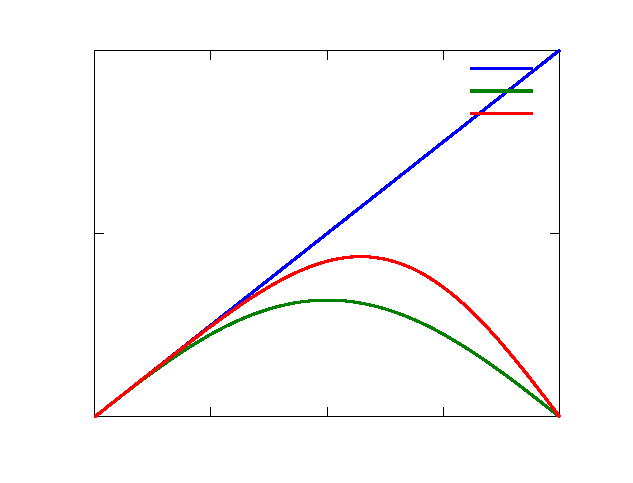
\includegraphics{scalfreq}}%
    \gplfronttext
  \end{picture}%
\endgroup
}
	\end{center}
	%
\end{frame}
%
%%%%%%%%%%%%%%%%%%%%%%%%%%%%%%%%%%%%%%%%%%%%%%%%%%%%%%%%%%%%%%%%%%%%%%
%
\begin{frame}
	%
	\frametitle{Phase speed}
	%
	\begin{center}
		\scalebox{.8}{% GNUPLOT: LaTeX picture with Postscript
\begingroup
  \makeatletter
  \providecommand\color[2][]{%
    \GenericError{(gnuplot) \space\space\space\@spaces}{%
      Package color not loaded in conjunction with
      terminal option `colourtext'%
    }{See the gnuplot documentation for explanation.%
    }{Either use 'blacktext' in gnuplot or load the package
      color.sty in LaTeX.}%
    \renewcommand\color[2][]{}%
  }%
  \providecommand\includegraphics[2][]{%
    \GenericError{(gnuplot) \space\space\space\@spaces}{%
      Package graphicx or graphics not loaded%
    }{See the gnuplot documentation for explanation.%
    }{The gnuplot epslatex terminal needs graphicx.sty or graphics.sty.}%
    \renewcommand\includegraphics[2][]{}%
  }%
  \providecommand\rotatebox[2]{#2}%
  \@ifundefined{ifGPcolor}{%
    \newif\ifGPcolor
    \GPcolortrue
  }{}%
  \@ifundefined{ifGPblacktext}{%
    \newif\ifGPblacktext
    \GPblacktexttrue
  }{}%
  % define a \g@addto@macro without @ in the name:
  \let\gplgaddtomacro\g@addto@macro
  % define empty templates for all commands taking text:
  \gdef\gplbacktext{}%
  \gdef\gplfronttext{}%
  \makeatother
  \ifGPblacktext
    % no textcolor at all
    \def\colorrgb#1{}%
    \def\colorgray#1{}%
  \else
    % gray or color?
    \ifGPcolor
      \def\colorrgb#1{\color[rgb]{#1}}%
      \def\colorgray#1{\color[gray]{#1}}%
      \expandafter\def\csname LTw\endcsname{\color{white}}%
      \expandafter\def\csname LTb\endcsname{\color{black}}%
      \expandafter\def\csname LTa\endcsname{\color{black}}%
      \expandafter\def\csname LT0\endcsname{\color[rgb]{1,0,0}}%
      \expandafter\def\csname LT1\endcsname{\color[rgb]{0,1,0}}%
      \expandafter\def\csname LT2\endcsname{\color[rgb]{0,0,1}}%
      \expandafter\def\csname LT3\endcsname{\color[rgb]{1,0,1}}%
      \expandafter\def\csname LT4\endcsname{\color[rgb]{0,1,1}}%
      \expandafter\def\csname LT5\endcsname{\color[rgb]{1,1,0}}%
      \expandafter\def\csname LT6\endcsname{\color[rgb]{0,0,0}}%
      \expandafter\def\csname LT7\endcsname{\color[rgb]{1,0.3,0}}%
      \expandafter\def\csname LT8\endcsname{\color[rgb]{0.5,0.5,0.5}}%
    \else
      % gray
      \def\colorrgb#1{\color{black}}%
      \def\colorgray#1{\color[gray]{#1}}%
      \expandafter\def\csname LTw\endcsname{\color{white}}%
      \expandafter\def\csname LTb\endcsname{\color{black}}%
      \expandafter\def\csname LTa\endcsname{\color{black}}%
      \expandafter\def\csname LT0\endcsname{\color{black}}%
      \expandafter\def\csname LT1\endcsname{\color{black}}%
      \expandafter\def\csname LT2\endcsname{\color{black}}%
      \expandafter\def\csname LT3\endcsname{\color{black}}%
      \expandafter\def\csname LT4\endcsname{\color{black}}%
      \expandafter\def\csname LT5\endcsname{\color{black}}%
      \expandafter\def\csname LT6\endcsname{\color{black}}%
      \expandafter\def\csname LT7\endcsname{\color{black}}%
      \expandafter\def\csname LT8\endcsname{\color{black}}%
    \fi
  \fi
  \setlength{\unitlength}{0.0500bp}%
  \begin{picture}(5760.00,4320.00)%
    \gplgaddtomacro\gplbacktext{%
      \colorrgb{0.00,0.00,0.00}%
      \put(617,475){\makebox(0,0)[r]{\strut{}0}}%
      \colorrgb{0.00,0.00,0.00}%
      \put(617,3676){\makebox(0,0)[r]{\strut{}$c$}}%
      \colorrgb{0.00,0.00,0.00}%
      \put(749,255){\makebox(0,0){\strut{}0}}%
      \colorrgb{0.00,0.00,0.00}%
      \put(1865,255){\makebox(0,0){\strut{}$\pi/4$}}%
      \colorrgb{0.00,0.00,0.00}%
      \put(2981,255){\makebox(0,0){\strut{}$\pi/2$}}%
      \colorrgb{0.00,0.00,0.00}%
      \put(4097,255){\makebox(0,0){\strut{}$3\pi/4$}}%
      \colorrgb{0.00,0.00,0.00}%
      \put(5213,255){\makebox(0,0){\strut{}$\pi$}}%
      \colorrgb{0.00,0.00,0.00}%
      \put(-21,2235){\rotatebox{90}{\makebox(0,0){\strut{}$\omega/k$}}}%
      \colorrgb{0.00,0.00,0.00}%
      \put(2981,-75){\makebox(0,0){\strut{}$k\Delta x$}}%
    }%
    \gplgaddtomacro\gplfronttext{%
      \csname LTb\endcsname%
      \put(4226,3823){\makebox(0,0)[r]{\strut{}Analytic}}%
      \csname LTb\endcsname%
      \put(4226,3603){\makebox(0,0)[r]{\strut{}2nd order}}%
      \csname LTb\endcsname%
      \put(4226,3383){\makebox(0,0)[r]{\strut{}4th order}}%
    }%
    \gplbacktext
    \put(0,0){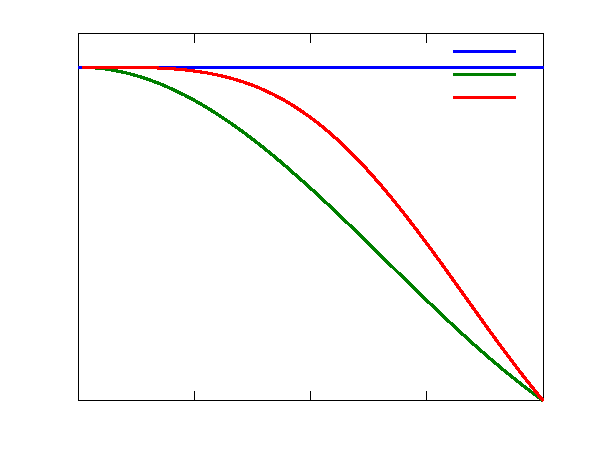
\includegraphics{phasespeed}}%
    \gplfronttext
  \end{picture}%
\endgroup
}
	\end{center}
	%
\end{frame}
%
%%%%%%%%%%%%%%%%%%%%%%%%%%%%%%%%%%%%%%%%%%%%%%%%%%%%%%%%%%%%%%%%%%%%%%
%
\begin{frame}
	%
	\frametitle{Group velocity}
	%
	\begin{center}
		\scalebox{.8}{% GNUPLOT: LaTeX picture with Postscript
\begingroup
  \makeatletter
  \providecommand\color[2][]{%
    \GenericError{(gnuplot) \space\space\space\@spaces}{%
      Package color not loaded in conjunction with
      terminal option `colourtext'%
    }{See the gnuplot documentation for explanation.%
    }{Either use 'blacktext' in gnuplot or load the package
      color.sty in LaTeX.}%
    \renewcommand\color[2][]{}%
  }%
  \providecommand\includegraphics[2][]{%
    \GenericError{(gnuplot) \space\space\space\@spaces}{%
      Package graphicx or graphics not loaded%
    }{See the gnuplot documentation for explanation.%
    }{The gnuplot epslatex terminal needs graphicx.sty or graphics.sty.}%
    \renewcommand\includegraphics[2][]{}%
  }%
  \providecommand\rotatebox[2]{#2}%
  \@ifundefined{ifGPcolor}{%
    \newif\ifGPcolor
    \GPcolortrue
  }{}%
  \@ifundefined{ifGPblacktext}{%
    \newif\ifGPblacktext
    \GPblacktexttrue
  }{}%
  % define a \g@addto@macro without @ in the name:
  \let\gplgaddtomacro\g@addto@macro
  % define empty templates for all commands taking text:
  \gdef\gplbacktext{}%
  \gdef\gplfronttext{}%
  \makeatother
  \ifGPblacktext
    % no textcolor at all
    \def\colorrgb#1{}%
    \def\colorgray#1{}%
  \else
    % gray or color?
    \ifGPcolor
      \def\colorrgb#1{\color[rgb]{#1}}%
      \def\colorgray#1{\color[gray]{#1}}%
      \expandafter\def\csname LTw\endcsname{\color{white}}%
      \expandafter\def\csname LTb\endcsname{\color{black}}%
      \expandafter\def\csname LTa\endcsname{\color{black}}%
      \expandafter\def\csname LT0\endcsname{\color[rgb]{1,0,0}}%
      \expandafter\def\csname LT1\endcsname{\color[rgb]{0,1,0}}%
      \expandafter\def\csname LT2\endcsname{\color[rgb]{0,0,1}}%
      \expandafter\def\csname LT3\endcsname{\color[rgb]{1,0,1}}%
      \expandafter\def\csname LT4\endcsname{\color[rgb]{0,1,1}}%
      \expandafter\def\csname LT5\endcsname{\color[rgb]{1,1,0}}%
      \expandafter\def\csname LT6\endcsname{\color[rgb]{0,0,0}}%
      \expandafter\def\csname LT7\endcsname{\color[rgb]{1,0.3,0}}%
      \expandafter\def\csname LT8\endcsname{\color[rgb]{0.5,0.5,0.5}}%
    \else
      % gray
      \def\colorrgb#1{\color{black}}%
      \def\colorgray#1{\color[gray]{#1}}%
      \expandafter\def\csname LTw\endcsname{\color{white}}%
      \expandafter\def\csname LTb\endcsname{\color{black}}%
      \expandafter\def\csname LTa\endcsname{\color{black}}%
      \expandafter\def\csname LT0\endcsname{\color{black}}%
      \expandafter\def\csname LT1\endcsname{\color{black}}%
      \expandafter\def\csname LT2\endcsname{\color{black}}%
      \expandafter\def\csname LT3\endcsname{\color{black}}%
      \expandafter\def\csname LT4\endcsname{\color{black}}%
      \expandafter\def\csname LT5\endcsname{\color{black}}%
      \expandafter\def\csname LT6\endcsname{\color{black}}%
      \expandafter\def\csname LT7\endcsname{\color{black}}%
      \expandafter\def\csname LT8\endcsname{\color{black}}%
    \fi
  \fi
  \setlength{\unitlength}{0.0500bp}%
  \begin{picture}(5760.00,4320.00)%
    \gplgaddtomacro\gplbacktext{%
      \colorrgb{0.00,0.00,0.00}%
      \put(617,475){\makebox(0,0)[r]{\strut{}$-2c$}}%
      \colorrgb{0.00,0.00,0.00}%
      \put(617,1611){\makebox(0,0)[r]{\strut{}$-c$}}%
      \colorrgb{0.00,0.00,0.00}%
      \put(617,2747){\makebox(0,0)[r]{\strut{}0}}%
      \colorrgb{0.00,0.00,0.00}%
      \put(617,3882){\makebox(0,0)[r]{\strut{}$c$}}%
      \colorrgb{0.00,0.00,0.00}%
      \put(749,255){\makebox(0,0){\strut{}0}}%
      \colorrgb{0.00,0.00,0.00}%
      \put(1865,255){\makebox(0,0){\strut{}$\pi/4$}}%
      \colorrgb{0.00,0.00,0.00}%
      \put(2981,255){\makebox(0,0){\strut{}$\pi/2$}}%
      \colorrgb{0.00,0.00,0.00}%
      \put(4097,255){\makebox(0,0){\strut{}$3\pi/4$}}%
      \colorrgb{0.00,0.00,0.00}%
      \put(5213,255){\makebox(0,0){\strut{}$\pi$}}%
      \colorrgb{0.00,0.00,0.00}%
      \put(-285,2235){\rotatebox{90}{\makebox(0,0){\strut{}$\partial\omega/\partial k$}}}%
      \colorrgb{0.00,0.00,0.00}%
      \put(2981,-75){\makebox(0,0){\strut{}$k\Delta x$}}%
    }%
    \gplgaddtomacro\gplfronttext{%
      \csname LTb\endcsname%
      \put(4226,3823){\makebox(0,0)[r]{\strut{}Analytic}}%
      \csname LTb\endcsname%
      \put(4226,3603){\makebox(0,0)[r]{\strut{}2nd order}}%
      \csname LTb\endcsname%
      \put(4226,3383){\makebox(0,0)[r]{\strut{}4th order}}%
    }%
    \gplbacktext
    \put(0,0){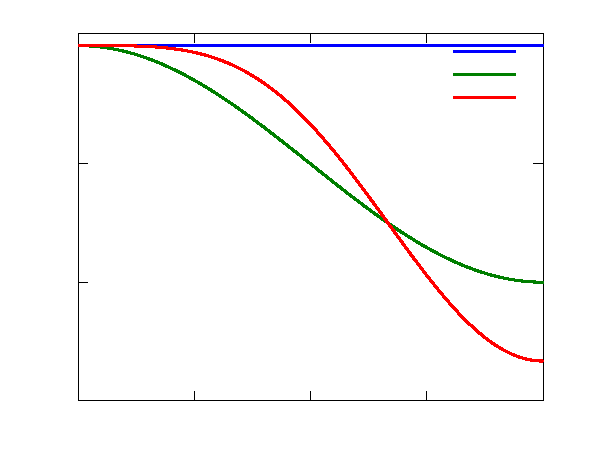
\includegraphics{groupvelocity}}%
    \gplfronttext
  \end{picture}%
\endgroup
}
	\end{center}
	%
\end{frame}
%
%%%%%%%%%%%%%%%%%%%%%%%%%%%%%%%%%%%%%%%%%%%%%%%%%%%%%%%%%%%%%%%%%%%%%%
%
\begin{frame}
	%
	\frametitle{A fundamental problem}
	%
	\vfill\begin{itemize}
		\item There is a fundamental problem with representing the phase of the $2\Delta x$ wave:
			%
			\begin{center}%
				\only<1>{%
					\scalebox{.8}{% GNUPLOT: LaTeX picture with Postscript
\begingroup
  \makeatletter
  \providecommand\color[2][]{%
    \GenericError{(gnuplot) \space\space\space\@spaces}{%
      Package color not loaded in conjunction with
      terminal option `colourtext'%
    }{See the gnuplot documentation for explanation.%
    }{Either use 'blacktext' in gnuplot or load the package
      color.sty in LaTeX.}%
    \renewcommand\color[2][]{}%
  }%
  \providecommand\includegraphics[2][]{%
    \GenericError{(gnuplot) \space\space\space\@spaces}{%
      Package graphicx or graphics not loaded%
    }{See the gnuplot documentation for explanation.%
    }{The gnuplot epslatex terminal needs graphicx.sty or graphics.sty.}%
    \renewcommand\includegraphics[2][]{}%
  }%
  \providecommand\rotatebox[2]{#2}%
  \@ifundefined{ifGPcolor}{%
    \newif\ifGPcolor
    \GPcolortrue
  }{}%
  \@ifundefined{ifGPblacktext}{%
    \newif\ifGPblacktext
    \GPblacktexttrue
  }{}%
  % define a \g@addto@macro without @ in the name:
  \let\gplgaddtomacro\g@addto@macro
  % define empty templates for all commands taking text:
  \gdef\gplbacktext{}%
  \gdef\gplfronttext{}%
  \makeatother
  \ifGPblacktext
    % no textcolor at all
    \def\colorrgb#1{}%
    \def\colorgray#1{}%
  \else
    % gray or color?
    \ifGPcolor
      \def\colorrgb#1{\color[rgb]{#1}}%
      \def\colorgray#1{\color[gray]{#1}}%
      \expandafter\def\csname LTw\endcsname{\color{white}}%
      \expandafter\def\csname LTb\endcsname{\color{black}}%
      \expandafter\def\csname LTa\endcsname{\color{black}}%
      \expandafter\def\csname LT0\endcsname{\color[rgb]{1,0,0}}%
      \expandafter\def\csname LT1\endcsname{\color[rgb]{0,1,0}}%
      \expandafter\def\csname LT2\endcsname{\color[rgb]{0,0,1}}%
      \expandafter\def\csname LT3\endcsname{\color[rgb]{1,0,1}}%
      \expandafter\def\csname LT4\endcsname{\color[rgb]{0,1,1}}%
      \expandafter\def\csname LT5\endcsname{\color[rgb]{1,1,0}}%
      \expandafter\def\csname LT6\endcsname{\color[rgb]{0,0,0}}%
      \expandafter\def\csname LT7\endcsname{\color[rgb]{1,0.3,0}}%
      \expandafter\def\csname LT8\endcsname{\color[rgb]{0.5,0.5,0.5}}%
    \else
      % gray
      \def\colorrgb#1{\color{black}}%
      \def\colorgray#1{\color[gray]{#1}}%
      \expandafter\def\csname LTw\endcsname{\color{white}}%
      \expandafter\def\csname LTb\endcsname{\color{black}}%
      \expandafter\def\csname LTa\endcsname{\color{black}}%
      \expandafter\def\csname LT0\endcsname{\color{black}}%
      \expandafter\def\csname LT1\endcsname{\color{black}}%
      \expandafter\def\csname LT2\endcsname{\color{black}}%
      \expandafter\def\csname LT3\endcsname{\color{black}}%
      \expandafter\def\csname LT4\endcsname{\color{black}}%
      \expandafter\def\csname LT5\endcsname{\color{black}}%
      \expandafter\def\csname LT6\endcsname{\color{black}}%
      \expandafter\def\csname LT7\endcsname{\color{black}}%
      \expandafter\def\csname LT8\endcsname{\color{black}}%
    \fi
  \fi
  \setlength{\unitlength}{0.0500bp}%
  \begin{picture}(5760.00,3600.00)%
    \gplgaddtomacro\gplbacktext{%
      \colorrgb{0.00,0.00,0.00}%
      \put(748,176){\makebox(0,0){\strut{}0}}%
      \colorrgb{0.00,0.00,0.00}%
      \put(1864,176){\makebox(0,0){\strut{}$\Delta x$}}%
      \colorrgb{0.00,0.00,0.00}%
      \put(2980,176){\makebox(0,0){\strut{}$2\Delta x$}}%
      \colorrgb{0.00,0.00,0.00}%
      \put(4096,176){\makebox(0,0){\strut{}$3\Delta x$}}%
      \colorrgb{0.00,0.00,0.00}%
      \put(5212,176){\makebox(0,0){\strut{}$4\Delta x$}}%
      \colorrgb{0.00,0.00,0.00}%
      \put(528,1862){\rotatebox{90}{\makebox(0,0){\strut{}$\cos\left(\frac{\pi}{\Delta x}x\right)$}}}%
      \colorrgb{0.00,0.00,0.00}%
      \put(2980,-153){\makebox(0,0){\strut{}$x$}}%
    }%
    \gplgaddtomacro\gplfronttext{%
    }%
    \gplbacktext
    \put(0,0){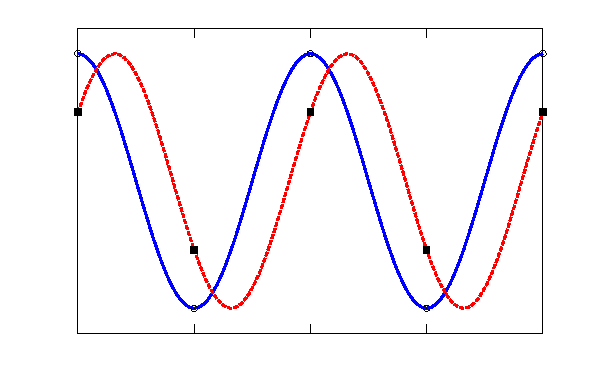
\includegraphics{phase2dx_1}}%
    \gplfronttext
  \end{picture}%
\endgroup
}%
				}%
				\only<2->{%
					\scalebox{.8}{% GNUPLOT: LaTeX picture with Postscript
\begingroup
  \makeatletter
  \providecommand\color[2][]{%
    \GenericError{(gnuplot) \space\space\space\@spaces}{%
      Package color not loaded in conjunction with
      terminal option `colourtext'%
    }{See the gnuplot documentation for explanation.%
    }{Either use 'blacktext' in gnuplot or load the package
      color.sty in LaTeX.}%
    \renewcommand\color[2][]{}%
  }%
  \providecommand\includegraphics[2][]{%
    \GenericError{(gnuplot) \space\space\space\@spaces}{%
      Package graphicx or graphics not loaded%
    }{See the gnuplot documentation for explanation.%
    }{The gnuplot epslatex terminal needs graphicx.sty or graphics.sty.}%
    \renewcommand\includegraphics[2][]{}%
  }%
  \providecommand\rotatebox[2]{#2}%
  \@ifundefined{ifGPcolor}{%
    \newif\ifGPcolor
    \GPcolortrue
  }{}%
  \@ifundefined{ifGPblacktext}{%
    \newif\ifGPblacktext
    \GPblacktexttrue
  }{}%
  % define a \g@addto@macro without @ in the name:
  \let\gplgaddtomacro\g@addto@macro
  % define empty templates for all commands taking text:
  \gdef\gplbacktext{}%
  \gdef\gplfronttext{}%
  \makeatother
  \ifGPblacktext
    % no textcolor at all
    \def\colorrgb#1{}%
    \def\colorgray#1{}%
  \else
    % gray or color?
    \ifGPcolor
      \def\colorrgb#1{\color[rgb]{#1}}%
      \def\colorgray#1{\color[gray]{#1}}%
      \expandafter\def\csname LTw\endcsname{\color{white}}%
      \expandafter\def\csname LTb\endcsname{\color{black}}%
      \expandafter\def\csname LTa\endcsname{\color{black}}%
      \expandafter\def\csname LT0\endcsname{\color[rgb]{1,0,0}}%
      \expandafter\def\csname LT1\endcsname{\color[rgb]{0,1,0}}%
      \expandafter\def\csname LT2\endcsname{\color[rgb]{0,0,1}}%
      \expandafter\def\csname LT3\endcsname{\color[rgb]{1,0,1}}%
      \expandafter\def\csname LT4\endcsname{\color[rgb]{0,1,1}}%
      \expandafter\def\csname LT5\endcsname{\color[rgb]{1,1,0}}%
      \expandafter\def\csname LT6\endcsname{\color[rgb]{0,0,0}}%
      \expandafter\def\csname LT7\endcsname{\color[rgb]{1,0.3,0}}%
      \expandafter\def\csname LT8\endcsname{\color[rgb]{0.5,0.5,0.5}}%
    \else
      % gray
      \def\colorrgb#1{\color{black}}%
      \def\colorgray#1{\color[gray]{#1}}%
      \expandafter\def\csname LTw\endcsname{\color{white}}%
      \expandafter\def\csname LTb\endcsname{\color{black}}%
      \expandafter\def\csname LTa\endcsname{\color{black}}%
      \expandafter\def\csname LT0\endcsname{\color{black}}%
      \expandafter\def\csname LT1\endcsname{\color{black}}%
      \expandafter\def\csname LT2\endcsname{\color{black}}%
      \expandafter\def\csname LT3\endcsname{\color{black}}%
      \expandafter\def\csname LT4\endcsname{\color{black}}%
      \expandafter\def\csname LT5\endcsname{\color{black}}%
      \expandafter\def\csname LT6\endcsname{\color{black}}%
      \expandafter\def\csname LT7\endcsname{\color{black}}%
      \expandafter\def\csname LT8\endcsname{\color{black}}%
    \fi
  \fi
  \setlength{\unitlength}{0.0500bp}%
  \begin{picture}(5760.00,3600.00)%
    \gplgaddtomacro\gplbacktext{%
      \colorrgb{0.00,0.00,0.00}%
      \put(748,176){\makebox(0,0){\strut{}0}}%
      \colorrgb{0.00,0.00,0.00}%
      \put(1864,176){\makebox(0,0){\strut{}$\Delta x$}}%
      \colorrgb{0.00,0.00,0.00}%
      \put(2980,176){\makebox(0,0){\strut{}$2\Delta x$}}%
      \colorrgb{0.00,0.00,0.00}%
      \put(4096,176){\makebox(0,0){\strut{}$3\Delta x$}}%
      \colorrgb{0.00,0.00,0.00}%
      \put(5212,176){\makebox(0,0){\strut{}$4\Delta x$}}%
      \colorrgb{0.00,0.00,0.00}%
      \put(528,1862){\rotatebox{90}{\makebox(0,0){\strut{}$\cos\left(\frac{\pi}{\Delta x}x\right)$}}}%
      \colorrgb{0.00,0.00,0.00}%
      \put(2980,-153){\makebox(0,0){\strut{}$x$}}%
    }%
    \gplgaddtomacro\gplfronttext{%
    }%
    \gplbacktext
    \put(0,0){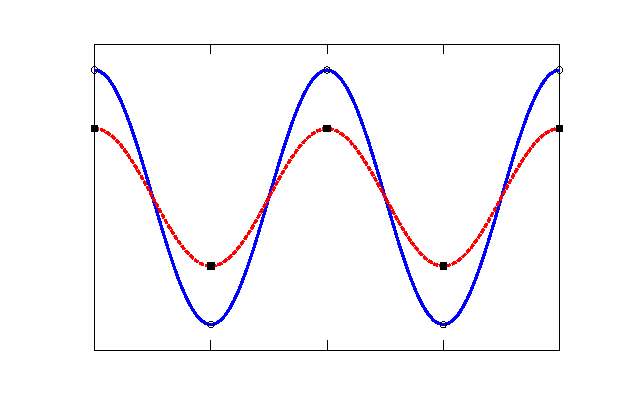
\includegraphics{phase2dx_2}}%
    \gplfronttext
  \end{picture}%
\endgroup
}%
				}%
			\end{center}%
			%
			\onslide<2->{%
				A phase shift looks like an amplitude change.
			}
	\end{itemize}\vfill
\end{frame}
%
%%%%%%%%%%%%%%%%%%%%%%%%%%%%%%%%%%%%%%%%%%%%%%%%%%%%%%%%%%%%%%%%%%%%%%
%
\begin{frame}
	%
	\frametitle{The spike test}
	%
	\vfill\begin{itemize}
		\item Advection of a sharp spike:
			%
			\begin{center}
				\scalebox{.8}{% GNUPLOT: LaTeX picture with Postscript
\begingroup
  \makeatletter
  \providecommand\color[2][]{%
    \GenericError{(gnuplot) \space\space\space\@spaces}{%
      Package color not loaded in conjunction with
      terminal option `colourtext'%
    }{See the gnuplot documentation for explanation.%
    }{Either use 'blacktext' in gnuplot or load the package
      color.sty in LaTeX.}%
    \renewcommand\color[2][]{}%
  }%
  \providecommand\includegraphics[2][]{%
    \GenericError{(gnuplot) \space\space\space\@spaces}{%
      Package graphicx or graphics not loaded%
    }{See the gnuplot documentation for explanation.%
    }{The gnuplot epslatex terminal needs graphicx.sty or graphics.sty.}%
    \renewcommand\includegraphics[2][]{}%
  }%
  \providecommand\rotatebox[2]{#2}%
  \@ifundefined{ifGPcolor}{%
    \newif\ifGPcolor
    \GPcolortrue
  }{}%
  \@ifundefined{ifGPblacktext}{%
    \newif\ifGPblacktext
    \GPblacktexttrue
  }{}%
  % define a \g@addto@macro without @ in the name:
  \let\gplgaddtomacro\g@addto@macro
  % define empty templates for all commands taking text:
  \gdef\gplbacktext{}%
  \gdef\gplfronttext{}%
  \makeatother
  \ifGPblacktext
    % no textcolor at all
    \def\colorrgb#1{}%
    \def\colorgray#1{}%
  \else
    % gray or color?
    \ifGPcolor
      \def\colorrgb#1{\color[rgb]{#1}}%
      \def\colorgray#1{\color[gray]{#1}}%
      \expandafter\def\csname LTw\endcsname{\color{white}}%
      \expandafter\def\csname LTb\endcsname{\color{black}}%
      \expandafter\def\csname LTa\endcsname{\color{black}}%
      \expandafter\def\csname LT0\endcsname{\color[rgb]{1,0,0}}%
      \expandafter\def\csname LT1\endcsname{\color[rgb]{0,1,0}}%
      \expandafter\def\csname LT2\endcsname{\color[rgb]{0,0,1}}%
      \expandafter\def\csname LT3\endcsname{\color[rgb]{1,0,1}}%
      \expandafter\def\csname LT4\endcsname{\color[rgb]{0,1,1}}%
      \expandafter\def\csname LT5\endcsname{\color[rgb]{1,1,0}}%
      \expandafter\def\csname LT6\endcsname{\color[rgb]{0,0,0}}%
      \expandafter\def\csname LT7\endcsname{\color[rgb]{1,0.3,0}}%
      \expandafter\def\csname LT8\endcsname{\color[rgb]{0.5,0.5,0.5}}%
    \else
      % gray
      \def\colorrgb#1{\color{black}}%
      \def\colorgray#1{\color[gray]{#1}}%
      \expandafter\def\csname LTw\endcsname{\color{white}}%
      \expandafter\def\csname LTb\endcsname{\color{black}}%
      \expandafter\def\csname LTa\endcsname{\color{black}}%
      \expandafter\def\csname LT0\endcsname{\color{black}}%
      \expandafter\def\csname LT1\endcsname{\color{black}}%
      \expandafter\def\csname LT2\endcsname{\color{black}}%
      \expandafter\def\csname LT3\endcsname{\color{black}}%
      \expandafter\def\csname LT4\endcsname{\color{black}}%
      \expandafter\def\csname LT5\endcsname{\color{black}}%
      \expandafter\def\csname LT6\endcsname{\color{black}}%
      \expandafter\def\csname LT7\endcsname{\color{black}}%
      \expandafter\def\csname LT8\endcsname{\color{black}}%
    \fi
  \fi
  \setlength{\unitlength}{0.0500bp}%
  \begin{picture}(5760.00,3600.00)%
    \gplgaddtomacro\gplbacktext{%
      \colorrgb{0.00,0.00,0.00}%
      \put(748,176){\makebox(0,0){\strut{}}}%
      \colorrgb{0.00,0.00,0.00}%
      \put(892,176){\makebox(0,0){\strut{}}}%
      \colorrgb{0.00,0.00,0.00}%
      \put(1036,176){\makebox(0,0){\strut{}}}%
      \colorrgb{0.00,0.00,0.00}%
      \put(1180,176){\makebox(0,0){\strut{}}}%
      \colorrgb{0.00,0.00,0.00}%
      \put(1324,176){\makebox(0,0){\strut{}}}%
      \colorrgb{0.00,0.00,0.00}%
      \put(1468,176){\makebox(0,0){\strut{}}}%
      \colorrgb{0.00,0.00,0.00}%
      \put(1612,176){\makebox(0,0){\strut{}}}%
      \colorrgb{0.00,0.00,0.00}%
      \put(1756,176){\makebox(0,0){\strut{}}}%
      \colorrgb{0.00,0.00,0.00}%
      \put(1900,176){\makebox(0,0){\strut{}}}%
      \colorrgb{0.00,0.00,0.00}%
      \put(2044,176){\makebox(0,0){\strut{}}}%
      \colorrgb{0.00,0.00,0.00}%
      \put(2188,176){\makebox(0,0){\strut{}}}%
      \colorrgb{0.00,0.00,0.00}%
      \put(2332,176){\makebox(0,0){\strut{}}}%
      \colorrgb{0.00,0.00,0.00}%
      \put(2476,176){\makebox(0,0){\strut{}}}%
      \colorrgb{0.00,0.00,0.00}%
      \put(2620,176){\makebox(0,0){\strut{}}}%
      \colorrgb{0.00,0.00,0.00}%
      \put(2764,176){\makebox(0,0){\strut{}}}%
      \colorrgb{0.00,0.00,0.00}%
      \put(2908,176){\makebox(0,0){\strut{}}}%
      \colorrgb{0.00,0.00,0.00}%
      \put(3052,176){\makebox(0,0){\strut{}}}%
      \colorrgb{0.00,0.00,0.00}%
      \put(3196,176){\makebox(0,0){\strut{}}}%
      \colorrgb{0.00,0.00,0.00}%
      \put(3340,176){\makebox(0,0){\strut{}}}%
      \colorrgb{0.00,0.00,0.00}%
      \put(3484,176){\makebox(0,0){\strut{}}}%
      \colorrgb{0.00,0.00,0.00}%
      \put(3628,176){\makebox(0,0){\strut{}}}%
      \colorrgb{0.00,0.00,0.00}%
      \put(3772,176){\makebox(0,0){\strut{}}}%
      \colorrgb{0.00,0.00,0.00}%
      \put(3916,176){\makebox(0,0){\strut{}}}%
      \colorrgb{0.00,0.00,0.00}%
      \put(4060,176){\makebox(0,0){\strut{}}}%
      \colorrgb{0.00,0.00,0.00}%
      \put(4204,176){\makebox(0,0){\strut{}}}%
      \colorrgb{0.00,0.00,0.00}%
      \put(4348,176){\makebox(0,0){\strut{}}}%
      \colorrgb{0.00,0.00,0.00}%
      \put(4492,176){\makebox(0,0){\strut{}}}%
      \colorrgb{0.00,0.00,0.00}%
      \put(4636,176){\makebox(0,0){\strut{}}}%
      \colorrgb{0.00,0.00,0.00}%
      \put(4780,176){\makebox(0,0){\strut{}}}%
      \colorrgb{0.00,0.00,0.00}%
      \put(4924,176){\makebox(0,0){\strut{}}}%
      \colorrgb{0.00,0.00,0.00}%
      \put(5068,176){\makebox(0,0){\strut{}}}%
      \colorrgb{0.00,0.00,0.00}%
      \put(5212,176){\makebox(0,0){\strut{}}}%
    }%
    \gplgaddtomacro\gplfronttext{%
      \csname LTb\endcsname%
      \put(4225,3156){\makebox(0,0)[r]{\strut{}exact}}%
      \csname LTb\endcsname%
      \put(4225,2936){\makebox(0,0)[r]{\strut{}2-c}}%
      \csname LTb\endcsname%
      \put(4225,2716){\makebox(0,0)[r]{\strut{}4-c}}%
    }%
    \gplbacktext
    \put(0,0){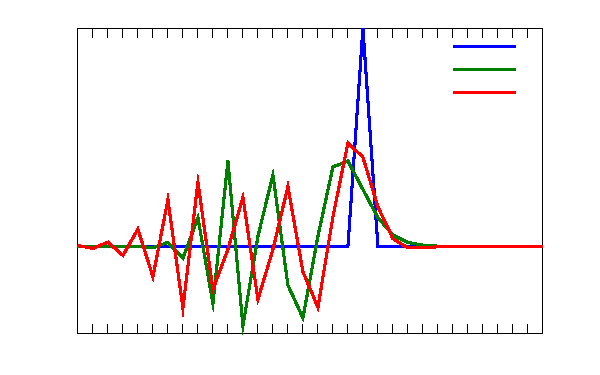
\includegraphics{spike_c}}%
    \gplfronttext
  \end{picture}%
\endgroup
}
			\end{center}
			%
	\end{itemize}\vfill
\end{frame}
%
%%%%%%%%%%%%%%%%%%%%%%%%%%%%%%%%%%%%%%%%%%%%%%%%%%%%%%%%%%%%%%%%%%%%%%
%
\begin{frame}
	%
	\frametitle{Decentered derivatives}
	%
	\vfill\begin{itemize}
		\item Let us try the one-sided decentered derivatives
			%
			\begin{equation*}
				\frac{d \phi_j}{dt} + c \left(\frac{\phi_j - \phi_{j-1}}{\Delta x} \right) =0
			\end{equation*}
			%
			which is the decentered scheme that we have seen before (upstream scheme).\vfill
			%
		\item The discrete dispersion relation becomes
			%
			\begin{equation*}
				\omega_{1s} = \frac{c}{i \Delta x} \left(1 - e^{- i k \Delta x}\right) 
					= \frac{c}{\Delta x}	\left[\sin k \Delta x +	i \left(\cos k \Delta x -1	\right)\right]
			\end{equation*}\vfill
			%
		\item Besides phase errors, there will be amplitude errors due to the imaginary part. The amplitude will grow or decay with a rate
			%
			\begin{equation*}
				\exp \left[ - \frac{c}{\Delta x} \left( 1 - \cos k \Delta x \right) t \right]
			\end{equation*}
			%
			In case $c<0$ this gives rise to an amplification, which is to be expected after what we saw in the first lesson.
			%
	\end{itemize}\vfill
\end{frame}
%
%%%%%%%%%%%%%%%%%%%%%%%%%%%%%%%%%%%%%%%%%%%%%%%%%%%%%%%%%%%%%%%%%%%%%%
%
\begin{frame}
	%
	\frametitle{Decentered derivatives}
	%
	\vfill\begin{itemize}
		\item Another one-sided decentered scheme is 
			%
			\begin{equation*}
				\frac{d \phi_j}{dt} + \ft16 c \frac{2 \phi_{j+1} + 3 \phi_j - 6 \phi_{j-1} + \phi_{j-2}}{\Delta x} = 0
			\end{equation*}
			%
			which is third-order.\vfill
			%
		\item The discrete dispersion relation becomes
			%
			\begin{equation*}
				\omega_{3s} = \frac{c}{\Delta x} \left[ \left( \ft43 \sin k \Delta x - \ft16 \sin 2 k \Delta x \right)
					- \ft{i}{3} \left( 1 - \cos k \Delta x	\right)^2 \right]
			\end{equation*}
			%
			which has the same phase error as the fourth-order scheme, and an amplitude decay
			%
			\begin{equation*}
				\exp \left[ - \frac{c}{3\Delta x} \left( 1 - \cos k \Delta x \right)^2 t \right]
			\end{equation*}
			%
	\end{itemize}\vfill
\end{frame}
%
%%%%%%%%%%%%%%%%%%%%%%%%%%%%%%%%%%%%%%%%%%%%%%%%%%%%%%%%%%%%%%%%%%%%%%
%
\begin{frame}
	%
	\frametitle{The spike test}
	%
	\vfill\begin{itemize}
		\item Advection of a sharp spike:
			%
			\begin{center}
				\scalebox{.8}{% GNUPLOT: LaTeX picture with Postscript
\begingroup
  \makeatletter
  \providecommand\color[2][]{%
    \GenericError{(gnuplot) \space\space\space\@spaces}{%
      Package color not loaded in conjunction with
      terminal option `colourtext'%
    }{See the gnuplot documentation for explanation.%
    }{Either use 'blacktext' in gnuplot or load the package
      color.sty in LaTeX.}%
    \renewcommand\color[2][]{}%
  }%
  \providecommand\includegraphics[2][]{%
    \GenericError{(gnuplot) \space\space\space\@spaces}{%
      Package graphicx or graphics not loaded%
    }{See the gnuplot documentation for explanation.%
    }{The gnuplot epslatex terminal needs graphicx.sty or graphics.sty.}%
    \renewcommand\includegraphics[2][]{}%
  }%
  \providecommand\rotatebox[2]{#2}%
  \@ifundefined{ifGPcolor}{%
    \newif\ifGPcolor
    \GPcolortrue
  }{}%
  \@ifundefined{ifGPblacktext}{%
    \newif\ifGPblacktext
    \GPblacktexttrue
  }{}%
  % define a \g@addto@macro without @ in the name:
  \let\gplgaddtomacro\g@addto@macro
  % define empty templates for all commands taking text:
  \gdef\gplbacktext{}%
  \gdef\gplfronttext{}%
  \makeatother
  \ifGPblacktext
    % no textcolor at all
    \def\colorrgb#1{}%
    \def\colorgray#1{}%
  \else
    % gray or color?
    \ifGPcolor
      \def\colorrgb#1{\color[rgb]{#1}}%
      \def\colorgray#1{\color[gray]{#1}}%
      \expandafter\def\csname LTw\endcsname{\color{white}}%
      \expandafter\def\csname LTb\endcsname{\color{black}}%
      \expandafter\def\csname LTa\endcsname{\color{black}}%
      \expandafter\def\csname LT0\endcsname{\color[rgb]{1,0,0}}%
      \expandafter\def\csname LT1\endcsname{\color[rgb]{0,1,0}}%
      \expandafter\def\csname LT2\endcsname{\color[rgb]{0,0,1}}%
      \expandafter\def\csname LT3\endcsname{\color[rgb]{1,0,1}}%
      \expandafter\def\csname LT4\endcsname{\color[rgb]{0,1,1}}%
      \expandafter\def\csname LT5\endcsname{\color[rgb]{1,1,0}}%
      \expandafter\def\csname LT6\endcsname{\color[rgb]{0,0,0}}%
      \expandafter\def\csname LT7\endcsname{\color[rgb]{1,0.3,0}}%
      \expandafter\def\csname LT8\endcsname{\color[rgb]{0.5,0.5,0.5}}%
    \else
      % gray
      \def\colorrgb#1{\color{black}}%
      \def\colorgray#1{\color[gray]{#1}}%
      \expandafter\def\csname LTw\endcsname{\color{white}}%
      \expandafter\def\csname LTb\endcsname{\color{black}}%
      \expandafter\def\csname LTa\endcsname{\color{black}}%
      \expandafter\def\csname LT0\endcsname{\color{black}}%
      \expandafter\def\csname LT1\endcsname{\color{black}}%
      \expandafter\def\csname LT2\endcsname{\color{black}}%
      \expandafter\def\csname LT3\endcsname{\color{black}}%
      \expandafter\def\csname LT4\endcsname{\color{black}}%
      \expandafter\def\csname LT5\endcsname{\color{black}}%
      \expandafter\def\csname LT6\endcsname{\color{black}}%
      \expandafter\def\csname LT7\endcsname{\color{black}}%
      \expandafter\def\csname LT8\endcsname{\color{black}}%
    \fi
  \fi
  \setlength{\unitlength}{0.0500bp}%
  \begin{picture}(5760.00,3600.00)%
    \gplgaddtomacro\gplbacktext{%
      \colorrgb{0.00,0.00,0.00}%
      \put(748,176){\makebox(0,0){\strut{}}}%
      \colorrgb{0.00,0.00,0.00}%
      \put(892,176){\makebox(0,0){\strut{}}}%
      \colorrgb{0.00,0.00,0.00}%
      \put(1036,176){\makebox(0,0){\strut{}}}%
      \colorrgb{0.00,0.00,0.00}%
      \put(1180,176){\makebox(0,0){\strut{}}}%
      \colorrgb{0.00,0.00,0.00}%
      \put(1324,176){\makebox(0,0){\strut{}}}%
      \colorrgb{0.00,0.00,0.00}%
      \put(1468,176){\makebox(0,0){\strut{}}}%
      \colorrgb{0.00,0.00,0.00}%
      \put(1612,176){\makebox(0,0){\strut{}}}%
      \colorrgb{0.00,0.00,0.00}%
      \put(1756,176){\makebox(0,0){\strut{}}}%
      \colorrgb{0.00,0.00,0.00}%
      \put(1900,176){\makebox(0,0){\strut{}}}%
      \colorrgb{0.00,0.00,0.00}%
      \put(2044,176){\makebox(0,0){\strut{}}}%
      \colorrgb{0.00,0.00,0.00}%
      \put(2188,176){\makebox(0,0){\strut{}}}%
      \colorrgb{0.00,0.00,0.00}%
      \put(2332,176){\makebox(0,0){\strut{}}}%
      \colorrgb{0.00,0.00,0.00}%
      \put(2476,176){\makebox(0,0){\strut{}}}%
      \colorrgb{0.00,0.00,0.00}%
      \put(2620,176){\makebox(0,0){\strut{}}}%
      \colorrgb{0.00,0.00,0.00}%
      \put(2764,176){\makebox(0,0){\strut{}}}%
      \colorrgb{0.00,0.00,0.00}%
      \put(2908,176){\makebox(0,0){\strut{}}}%
      \colorrgb{0.00,0.00,0.00}%
      \put(3052,176){\makebox(0,0){\strut{}}}%
      \colorrgb{0.00,0.00,0.00}%
      \put(3196,176){\makebox(0,0){\strut{}}}%
      \colorrgb{0.00,0.00,0.00}%
      \put(3340,176){\makebox(0,0){\strut{}}}%
      \colorrgb{0.00,0.00,0.00}%
      \put(3484,176){\makebox(0,0){\strut{}}}%
      \colorrgb{0.00,0.00,0.00}%
      \put(3628,176){\makebox(0,0){\strut{}}}%
      \colorrgb{0.00,0.00,0.00}%
      \put(3772,176){\makebox(0,0){\strut{}}}%
      \colorrgb{0.00,0.00,0.00}%
      \put(3916,176){\makebox(0,0){\strut{}}}%
      \colorrgb{0.00,0.00,0.00}%
      \put(4060,176){\makebox(0,0){\strut{}}}%
      \colorrgb{0.00,0.00,0.00}%
      \put(4204,176){\makebox(0,0){\strut{}}}%
      \colorrgb{0.00,0.00,0.00}%
      \put(4348,176){\makebox(0,0){\strut{}}}%
      \colorrgb{0.00,0.00,0.00}%
      \put(4492,176){\makebox(0,0){\strut{}}}%
      \colorrgb{0.00,0.00,0.00}%
      \put(4636,176){\makebox(0,0){\strut{}}}%
      \colorrgb{0.00,0.00,0.00}%
      \put(4780,176){\makebox(0,0){\strut{}}}%
      \colorrgb{0.00,0.00,0.00}%
      \put(4924,176){\makebox(0,0){\strut{}}}%
      \colorrgb{0.00,0.00,0.00}%
      \put(5068,176){\makebox(0,0){\strut{}}}%
      \colorrgb{0.00,0.00,0.00}%
      \put(5212,176){\makebox(0,0){\strut{}}}%
    }%
    \gplgaddtomacro\gplfronttext{%
      \csname LTb\endcsname%
      \put(4225,3156){\makebox(0,0)[r]{\strut{}exact}}%
      \csname LTb\endcsname%
      \put(4225,2936){\makebox(0,0)[r]{\strut{}1-s}}%
      \csname LTb\endcsname%
      \put(4225,2716){\makebox(0,0)[r]{\strut{}3-s}}%
    }%
    \gplbacktext
    \put(0,0){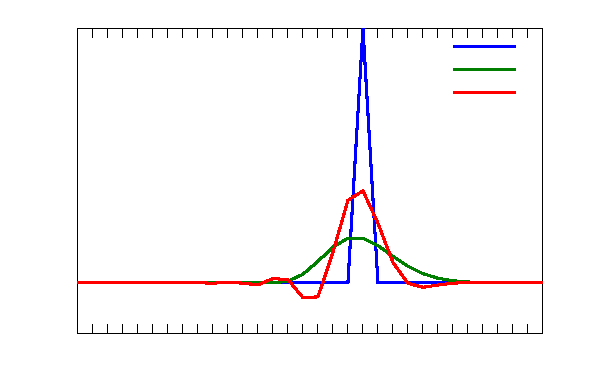
\includegraphics{spike_s}}%
    \gplfronttext
  \end{picture}%
\endgroup
}
			\end{center}
			%
	\end{itemize}\vfill
\end{frame}
%
%%%%%%%%%%%%%%%%%%%%%%%%%%%%%%%%%%%%%%%%%%%%%%%%%%%%%%%%%%%%%%%%%%%%%%
%
\begin{frame}
	%
	\frametitle{A more realistic test}
	%
	\vfill\begin{itemize}
		\item Advection of a sum of two waves:
			%
			\begin{center}
				\scalebox{.8}{% GNUPLOT: LaTeX picture with Postscript
\begingroup
  \makeatletter
  \providecommand\color[2][]{%
    \GenericError{(gnuplot) \space\space\space\@spaces}{%
      Package color not loaded in conjunction with
      terminal option `colourtext'%
    }{See the gnuplot documentation for explanation.%
    }{Either use 'blacktext' in gnuplot or load the package
      color.sty in LaTeX.}%
    \renewcommand\color[2][]{}%
  }%
  \providecommand\includegraphics[2][]{%
    \GenericError{(gnuplot) \space\space\space\@spaces}{%
      Package graphicx or graphics not loaded%
    }{See the gnuplot documentation for explanation.%
    }{The gnuplot epslatex terminal needs graphicx.sty or graphics.sty.}%
    \renewcommand\includegraphics[2][]{}%
  }%
  \providecommand\rotatebox[2]{#2}%
  \@ifundefined{ifGPcolor}{%
    \newif\ifGPcolor
    \GPcolortrue
  }{}%
  \@ifundefined{ifGPblacktext}{%
    \newif\ifGPblacktext
    \GPblacktexttrue
  }{}%
  % define a \g@addto@macro without @ in the name:
  \let\gplgaddtomacro\g@addto@macro
  % define empty templates for all commands taking text:
  \gdef\gplbacktext{}%
  \gdef\gplfronttext{}%
  \makeatother
  \ifGPblacktext
    % no textcolor at all
    \def\colorrgb#1{}%
    \def\colorgray#1{}%
  \else
    % gray or color?
    \ifGPcolor
      \def\colorrgb#1{\color[rgb]{#1}}%
      \def\colorgray#1{\color[gray]{#1}}%
      \expandafter\def\csname LTw\endcsname{\color{white}}%
      \expandafter\def\csname LTb\endcsname{\color{black}}%
      \expandafter\def\csname LTa\endcsname{\color{black}}%
      \expandafter\def\csname LT0\endcsname{\color[rgb]{1,0,0}}%
      \expandafter\def\csname LT1\endcsname{\color[rgb]{0,1,0}}%
      \expandafter\def\csname LT2\endcsname{\color[rgb]{0,0,1}}%
      \expandafter\def\csname LT3\endcsname{\color[rgb]{1,0,1}}%
      \expandafter\def\csname LT4\endcsname{\color[rgb]{0,1,1}}%
      \expandafter\def\csname LT5\endcsname{\color[rgb]{1,1,0}}%
      \expandafter\def\csname LT6\endcsname{\color[rgb]{0,0,0}}%
      \expandafter\def\csname LT7\endcsname{\color[rgb]{1,0.3,0}}%
      \expandafter\def\csname LT8\endcsname{\color[rgb]{0.5,0.5,0.5}}%
    \else
      % gray
      \def\colorrgb#1{\color{black}}%
      \def\colorgray#1{\color[gray]{#1}}%
      \expandafter\def\csname LTw\endcsname{\color{white}}%
      \expandafter\def\csname LTb\endcsname{\color{black}}%
      \expandafter\def\csname LTa\endcsname{\color{black}}%
      \expandafter\def\csname LT0\endcsname{\color{black}}%
      \expandafter\def\csname LT1\endcsname{\color{black}}%
      \expandafter\def\csname LT2\endcsname{\color{black}}%
      \expandafter\def\csname LT3\endcsname{\color{black}}%
      \expandafter\def\csname LT4\endcsname{\color{black}}%
      \expandafter\def\csname LT5\endcsname{\color{black}}%
      \expandafter\def\csname LT6\endcsname{\color{black}}%
      \expandafter\def\csname LT7\endcsname{\color{black}}%
      \expandafter\def\csname LT8\endcsname{\color{black}}%
    \fi
  \fi
  \setlength{\unitlength}{0.0500bp}%
  \begin{picture}(5760.00,3600.00)%
    \gplgaddtomacro\gplbacktext{%
      \colorrgb{0.00,0.00,0.00}%
      \put(748,176){\makebox(0,0){\strut{}}}%
      \colorrgb{0.00,0.00,0.00}%
      \put(902,176){\makebox(0,0){\strut{}}}%
      \colorrgb{0.00,0.00,0.00}%
      \put(1056,176){\makebox(0,0){\strut{}}}%
      \colorrgb{0.00,0.00,0.00}%
      \put(1210,176){\makebox(0,0){\strut{}}}%
      \colorrgb{0.00,0.00,0.00}%
      \put(1364,176){\makebox(0,0){\strut{}}}%
      \colorrgb{0.00,0.00,0.00}%
      \put(1518,176){\makebox(0,0){\strut{}}}%
      \colorrgb{0.00,0.00,0.00}%
      \put(1672,176){\makebox(0,0){\strut{}}}%
      \colorrgb{0.00,0.00,0.00}%
      \put(1826,176){\makebox(0,0){\strut{}}}%
      \colorrgb{0.00,0.00,0.00}%
      \put(1979,176){\makebox(0,0){\strut{}}}%
      \colorrgb{0.00,0.00,0.00}%
      \put(2133,176){\makebox(0,0){\strut{}}}%
      \colorrgb{0.00,0.00,0.00}%
      \put(2287,176){\makebox(0,0){\strut{}}}%
      \colorrgb{0.00,0.00,0.00}%
      \put(2441,176){\makebox(0,0){\strut{}}}%
      \colorrgb{0.00,0.00,0.00}%
      \put(2595,176){\makebox(0,0){\strut{}}}%
      \colorrgb{0.00,0.00,0.00}%
      \put(2749,176){\makebox(0,0){\strut{}}}%
      \colorrgb{0.00,0.00,0.00}%
      \put(2903,176){\makebox(0,0){\strut{}}}%
      \colorrgb{0.00,0.00,0.00}%
      \put(3057,176){\makebox(0,0){\strut{}}}%
      \colorrgb{0.00,0.00,0.00}%
      \put(3211,176){\makebox(0,0){\strut{}}}%
      \colorrgb{0.00,0.00,0.00}%
      \put(3365,176){\makebox(0,0){\strut{}}}%
      \colorrgb{0.00,0.00,0.00}%
      \put(3519,176){\makebox(0,0){\strut{}}}%
      \colorrgb{0.00,0.00,0.00}%
      \put(3673,176){\makebox(0,0){\strut{}}}%
      \colorrgb{0.00,0.00,0.00}%
      \put(3827,176){\makebox(0,0){\strut{}}}%
      \colorrgb{0.00,0.00,0.00}%
      \put(3981,176){\makebox(0,0){\strut{}}}%
      \colorrgb{0.00,0.00,0.00}%
      \put(4134,176){\makebox(0,0){\strut{}}}%
      \colorrgb{0.00,0.00,0.00}%
      \put(4288,176){\makebox(0,0){\strut{}}}%
      \colorrgb{0.00,0.00,0.00}%
      \put(4442,176){\makebox(0,0){\strut{}}}%
      \colorrgb{0.00,0.00,0.00}%
      \put(4596,176){\makebox(0,0){\strut{}}}%
      \colorrgb{0.00,0.00,0.00}%
      \put(4750,176){\makebox(0,0){\strut{}}}%
      \colorrgb{0.00,0.00,0.00}%
      \put(4904,176){\makebox(0,0){\strut{}}}%
      \colorrgb{0.00,0.00,0.00}%
      \put(5058,176){\makebox(0,0){\strut{}}}%
      \colorrgb{0.00,0.00,0.00}%
      \put(5212,176){\makebox(0,0){\strut{}}}%
    }%
    \gplgaddtomacro\gplfronttext{%
      \csname LTb\endcsname%
      \put(4225,3156){\makebox(0,0)[r]{\strut{}exact}}%
      \csname LTb\endcsname%
      \put(4225,2936){\makebox(0,0)[r]{\strut{}1-s}}%
      \csname LTb\endcsname%
      \put(4225,2716){\makebox(0,0)[r]{\strut{}2-c}}%
      \csname LTb\endcsname%
      \put(4225,2496){\makebox(0,0)[r]{\strut{}3-s}}%
      \csname LTb\endcsname%
      \put(4225,2276){\makebox(0,0)[r]{\strut{}4-c}}%
    }%
    \gplbacktext
    \put(0,0){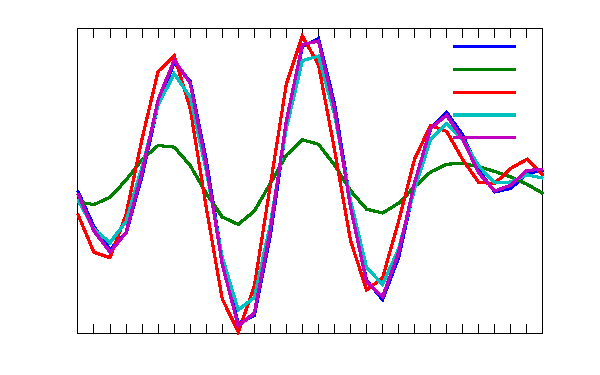
\includegraphics{two_wave}}%
    \gplfronttext
  \end{picture}%
\endgroup
}
			\end{center}
			%
	\end{itemize}\vfill
\end{frame}
%
%%%%%%%%%%%%%%%%%%%%%%%%%%%%%%%%%%%%%%%%%%%%%%%%%%%%%%%%%%%%%%%%%%%%%%
%
\begin{frame}
	%
	\frametitle{Discussion}
	%
	\vfill\begin{itemize}
		\item The damping in the decentered schemes can be good or bad;\vfill
		\item In the spike test they damp the spurious trail which makes decentered schemes actually better than the centered ones.\vfill
		\item The third-order scheme somewhat better approximates the analytic solution than the first-order one\vfill
		\item However, the spike test is an extreme test! In the more realistic test with 2 modes it is not clear whether the third-order decentered scheme is better than the second-order centered one:\vspace*{1ex}
			\begin{itemize}
				\item The amplitude is better for the second-order one
				\item The third-order one does not make a phase error.
			\end{itemize}
	\end{itemize}\vfill
	%
\end{frame}
%
%%%%%%%%%%%%%%%%%%%%%%%%%%%%%%%%%%%%%%%%%%%%%%%%%%%%%%%%%%%%%%%%%%%%%%
%
\begin{frame}
	%
	\frametitle{Dissipation and dispersion}
	%
	\vfill\begin{itemize}
		\item A qualitative description of the error is obtained by examining the truncated terms; instead of solving the advection equation with zero RHS, we are in fact solving
			%
			\begin{equation*}
				\frac{\partial \phi}{\partial t}+c\frac{\partial \phi}{\partial x}=
					\epsilon_m\frac{\partial^m \phi}{\partial x^m}+
					\epsilon_{m+1}\frac{\partial^{m+1} \phi}{\partial x^{m+1}}+\ldots
			\end{equation*}\vfill
			%
		\item an even order $m$ will lead to a dissipative effect:
			%
			\begin{equation*}
				\frac{\partial \xi}{\partial t} = \frac{\partial^{m} \xi}{\partial x^{m}}
					\quad\Rightarrow\quad\xi (x,t) = C e^{ikx} e^{-\gamma t}
			\end{equation*}\vfill
			%
		\item an odd term will lead to a dispersive effect:
			%
			\begin{equation*}
				\frac{\partial \xi}{\partial t} = \frac{\partial^m \xi}{\partial x^m}
					\quad\Rightarrow\quad\xi (x,t) = C e^{i \left( kx - \omega t \right)}
			\end{equation*}
			%
	\end{itemize}\vfill
	%
\end{frame}
%
%%%%%%%%%%%%%%%%%%%%%%%%%%%%%%%%%%%%%%%%%%%%%%%%%%%%%%%%%%%%%%%%%%%%%%
%
\begin{frame}
	%
	\frametitle{Discussion}
	%
	\vfill\begin{itemize}
		\item The centered derivatives have \emph{no} numerical dissipation.\\
			(only odd terms in the truncation error)\vfill
			%
		\item The first and second-order have the same leading-order dispersive terms, so they have the same dispersion! The same holds for the third- and fourth order schemes.\vspace*{2ex}
			%
		\item In fact, the dispersive error in the odd-order schemes are dissipated away!\vfill
			%
		\item So we are compensating one error by another! This is usually a bad idea.\vfill
			%
		\item One way out for the even-order schemes is to introduce some (controlled) artificial dissipation.\vfill
			%
		\item (We will see later that this is in fact also important in nonlinear systems).
			%
	\end{itemize}\vfill
	%
\end{frame}
%
%%%%%%%%%%%%%%%%%%%%%%%%%%%%%%%%%%%%%%%%%%%%%%%%%%%%%%%%%%%%%%%%%%%%%%
%
\begin{frame}
	%
	\frametitle{Time and space differencing}
	%
	\vfill\begin{itemize}
		\item Until now we have been isolating the error coming from the \emph{time differencing} and the \emph{space differencing}\vfill
			%
		\item The \emph{fundamental} behaviour of the scheme can sometimes be deduced from the constituents.\vfill
			%
			\par
			For instance, a combination of a \emph{forward difference scheme} with \emph{centered derivatives} will be a combination of an amplifying time scheme with a neutral space scheme, yielding an amplifying scheme.\vfill
			%
		\item But what will happen if we combine \emph{forward differencing} with an \emph{upstream one-sided space differencing}? Forward differencing will amplify, while the one-side space differencing may damp the mode. Further analysis is needed\ldots\vfill
			%
		\item What if we combine the leapfrog scheme with centered space differencing? Leapfrog is conditionally neutral; centered-space differencing is neutral. But leapfrog is accelerating, whereas centered differencing is decelarating?
			%
	\end{itemize}\vfill
\end{frame}
%
%%%%%%%%%%%%%%%%%%%%%%%%%%%%%%%%%%%%%%%%%%%%%%%%%%%%%%%%%%%%%%%%%%%%%%
%
\begin{frame}
	%
	\frametitle{Discrete dispersion relation}
	%
	\vfill\begin{itemize}
		\item One can consider the solution to the time- and space-discretized equation of the form
			%
			\begin{equation*}
				\phi_j^n = e^{i \left( k j \Delta x - \omega n \Delta t \right)}
			\end{equation*}
			%
		\item Substituting this solution in the scheme and solving for $\omega$ as a function of $k$ gives the \emph{discrete dispersion relation}.\vfill
			%
		\item In fact, it summarizes the behaviour of a scheme completely: let $\omega = \omega_r + i \omega_i$, then\vfill
			%
			\begin{itemize}
				\item $\omega_i$ determines the amplification factor\vfill
				\item $\omega_r$ determines the phase-speed error.\vfill
			\end{itemize}
			%
			(leave the complex algebra to a computer or a mathematician\ldots)
			%
	\end{itemize}\vfill
\end{frame}
%
%%%%%%%%%%%%%%%%%%%%%%%%%%%%%%%%%%%%%%%%%%%%%%%%%%%%%%%%%%%%%%%%%%%%%%
%
\begin{frame}
	%
	\frametitle{Summary}
	%
	\vfill\begin{itemize}
		\item We studied the influence of space discretization through the \emph{dispersion relation}\vfill
		\item The dispersion relation tells how waves propagate; phase speed and group speed.\vfill
		\item All finite difference schemes have difficulties with the $2\Delta x$ wave\vfill
		\item Decentered schemes also show damping, on top of dispersion\vfill
		\item Also combined time-space effects can be studied through the dispersion relation
	\end{itemize}\vfill
	%
\end{frame}
%
%%%%%%%%%%%%%%%%%%%%%%%%%%%%%%%%%%%%%%%%%%%%%%%%%%%%%%%%%%%%%%%%%%%%%%
%
\begin{frame}
	%
	\frametitle{Exercises}
	%
	\begin{enumerate}
		\item Determine the discrete dispersion relation for a 2nd-order centered leapfrog discretization of the advection equation:
			%
			\begin{equation*}
				\frac{\phi_j^{n+1}-\phi_j^{n-1}}{2\Delta t}+c\frac{\phi^n_{j+1}-\phi^n_{j-1}}{2\Delta x}=0
			\end{equation*}
			%
			You'll need $\frac{e^{i\theta}-e^{-i\theta}}{2i}=\sin\theta$.\vspace*{6ex}
		\item Determine the discrete dispersion relation for the upstream scheme:
			\begin{equation*}
				\frac{\phi_j^{n+1}-\phi_j^{n}}{\Delta t}+c\frac{\phi^n_{j}-\phi^n_{j-1}}{\Delta x}=0
			\end{equation*}
			%
			You'll need $\log (a+ib)=\frac{1}{2}\log(a^2+b^2)+i\,\arctan(b,a)$. This is pretty hard to calculate analytically, so use a computer to check the results\ldots
			%
			%[you'll need log(a+ib)=log(a^2+b^2)/2+i*atan2(b,a)]
			%
			%w=i/dt*log[1+mu*(cos+i*sin)] = wr+i*wi
			%	
			%so 
			%
			%wi=1/2*log((1+mu*cos-mu)^2+(mu*sin)^2)
			%
			%wi>0 	<=> 	1+(mu*cos)^2+mu^2+2*mu*cos-2*mu^2*cos-2*mu+(mu*sin)^2 < 1
			%			<=>		mu^2+mu*cos-mu^2*cos-mu < 0 
			%			<=>		mu*(mu-1)*(1-cos) < 0
			%			<=>		0 < mu < 1
			%			
			%Q.E.D
			%
			%(pretty hard to do analytically, so use a computer to visualize the result)
			%
			\par
			Does this confirm what we saw in the first lesson?
	\end{enumerate}
\end{frame}
%
%%%%%%%%%%%%%%%%%%%%%%%%%%%%%%%%%%%%%%%%%%%%%%%%%%%%%%%%%%%%%%%%%%%%%%
%
\begin{frame}
	%
	\frametitle{Exercises: Leapfrog, 2nd order FD}
	%
	\begin{equation*}
		\frac{\phi_j^{n+1}-\phi_j^{n-1}}{2\Delta t}+c\frac{\phi^n_{j+1}-\phi^n_{j-1}}{2\Delta x}=0
	\end{equation*}
	%
\pause
	Substituting a harmonic solution, discretized in space and time: $\phi_j^n=e^{i(kj\Delta x-\omega n \Delta t)}$, gives:
	%
	\begin{equation*}
		\frac{e^{i(kj\Delta x-\omega (n+1)\Delta t)}-e^{i(kj\Delta x-\omega (n-1)\Delta t)}}{2\Delta t}+c\frac{e^{i(k(j+1)\Delta x-\omega n\Delta t)}-e^{i(k(j-1)\Delta x-\omega n\Delta t)}}{2\Delta x}=0
	\end{equation*}	
	%
\pause
	Dividing both sides by $e^{i(kj\Delta x-\omega n\Delta t)}$, gives:
	\begin{equation*}
		\frac{e^{-i\omega\Delta t}-e^{i\omega\Delta t}}{2\Delta t}+c\frac{e^{ik\Delta x}-e^{-ik\Delta x}}{2\Delta x}=0
	\end{equation*}
\pause
	Using $e^{i\theta}-e^{-i\theta}=2i\sin\theta$, this is simplified to
	\begin{equation*}
		\sin\omega\Delta t=\frac{c\Delta t}{\Delta x}\sin k\Delta x
	\end{equation*}
\end{frame}
%
%%%%%%%%%%%%%%%%%%%%%%%%%%%%%%%%%%%%%%%%%%%%%%%%%%%%%%%%%%%%%%%%%%%%%%
%
\begin{frame}
	%
	\frametitle{Exercises: Leapfrog, 2nd order FD}
	%
	The discrete dispersion relation is 
	%
	\begin{equation*}
		\omega=\frac{1}{\Delta t}\arcsin\left(\frac{c\Delta t}{\Delta x}\sin k\Delta x\right)
	\end{equation*}
	%
	So:
	\begin{itemize}
		\item for $\left|\frac{c\Delta t}{\Delta x}\right|<1$, $\omega$ is real. The scheme is stable without amplitude error.
		\item for $\left|\frac{c\Delta t}{\Delta x}\right|>1$, $\omega$ is complex. The scheme is unstable.
		\item for $k\Delta x=\pi$, $\omega=0$. So the scheme is decelerating.
	\end{itemize}
	%
\end{frame}
%
%%%%%%%%%%%%%%%%%%%%%%%%%%%%%%%%%%%%%%%%%%%%%%%%%%%%%%%%%%%%%%%%%%%%%%
%
\begin{frame}
	%
	\frametitle{Exercises: upstream scheme}
	%
	\begin{equation*}
		\frac{\phi_j^{n+1}-\phi_j^{n}}{\Delta t}+c\frac{\phi^n_{j}-\phi^n_{j-1}}{\Delta x}=0
	\end{equation*}
	%
\pause
	Substituting a harmonic solution, discretized in space and time: $\phi_j^n=e^{i(kj\Delta x-\omega n \Delta t)}$, and dividing both sides by $\phi_j^n$, gives:
	%
	\begin{equation*}
		e^{-i\omega\Delta t}-1+\frac{c\Delta t}{\Delta x}\left(1-e^{-ik\Delta x}\right)=0
	\end{equation*}
	%
\pause
	The discrete dispersion relation becomes
	%
	\begin{equation*}
		\omega=\frac{i}{\Delta t}\log\left(1-\mu\left(1-\cos k\Delta x+i\sin k\Delta x\right)\right)
	\end{equation*}
	%
	with $\mu$ the Courant number $\mu=\frac{c\Delta t}{\Delta x}$.
\end{frame}
%
%%%%%%%%%%%%%%%%%%%%%%%%%%%%%%%%%%%%%%%%%%%%%%%%%%%%%%%%%%%%%%%%%%%%%%
%
\begin{frame}
	%
	\frametitle{Exercises: upstream scheme}
	%
	Stability is obtained if the imaginary part of $\omega$ is smaller than zero, i.e. if
	%
	\begin{equation*}
		\log\left(\left(1-\mu+\mu\cos k\Delta x\right)^2+\left(\mu\sin k\Delta x\right)^2\right) \leq 0
	\end{equation*}
	%
\pause
	This is equivalent to
	%
	\begin{equation*}
		\left(\left(1-\mu+\mu\cos k\Delta x\right)^2+\left(\mu\sin k\Delta x\right)^2\right) \leq 1
	\end{equation*}
	%
\pause
	Or
	\begin{equation*}
		\mu(1-\mu)(1-\cos k\Delta x) \leq 0
	\end{equation*}
	%
\pause
	Since $|\cos k\Delta x|\leq 1$, stability is guaranteed if
	%
	\begin{equation*}
		\mu(1-\mu) \leq 0
	\end{equation*}
	%
\pause
	Or if
	\begin{equation*}
		0\leq \mu\leq 1
	\end{equation*}
	%
\end{frame}
%
%%%%%%%%%%%%%%%%%%%%%%%%%%%%%%%%%%%%%%%%%%%%%%%%%%%%%%%%%%%%%%%%%%%%%%
%
\end{document}


